\chapter{Literature Review}
\label{ch_literature}

\section{Optics}

\subsection{Brief History}
Optics as defined by the Oxford English Dictionary is "The branch of physics that deals with the properties and phenomena of visible light (and by extension other forms of electromagnetic radiation), sometimes esp. in relation to sight." \cite{oed}.

For most of human history, little was known of the complex phenomena we call light. The first attempts to understand the properties of light were philosophical and history tells us that the Greek philosophers took interest in the subject. Around 300BC Euclid postulated that light propagated in a rectilinear fashion. He also stated the law of reflection. These principles still form part of our understanding of light today. \cite{Vohnsen_2004}

Well before any established scientific theories existed, lenses and their optical properties have been used for visual aid both for visually impaired persons and for magnification of objects. It was however only in the 17th century that the first record of telescopes can be found. Galileo is the first to record the use of such devices for the purpose of scientific inquiry.

In the 17th century scientist Descartes recorded his corpuscular theory of light. This theory was supported and further developed by Newton. In the same century Snell developed what we now know as Snell's law of refraction.

TBC.

\subsection{Optical Communication}

Optical communication concerns all manors of communicating information from one party to another through the medium of light. This investigation focuses on the use of light as a means of communication between electronic systems, however it is worth noting that optical communication certainly exist outside of this category.

\subsection{Lenses}
%todo: work on the image presentation format (subfigures)
This projects requires the use of a lens to focus a source of light into a narrow beam. Lenses work on the principle of refraction. When light enters a medium with a different refractive index at an angle offset from the perpendicular (normal), the light is bent toward or away from the normal, behaviour described by Snell's law.

When working with lenses, the lens equation may be used to determine how an object might form a real image or virtual image when viewed through a lens \cite{Knight2013}, however for the purposes of our investigation the definition of the focal length is sufficient.

\begin{figure}[H]
	\centering
	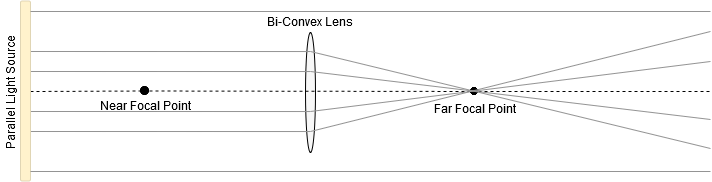
\includegraphics[width=0.8\linewidth]{figures/litreview/lens_diagram.png}
	\caption{Focal Point Illustration}
	\label{fig:lens_diagram}
\end{figure}

Figure \ref{fig:lens_diagram} above shows the near and far focal points for a lens. The diagram illustrates the behaviour of light rays produced by a theoretical parallel light source and passing through a bi-convex lens. The focal point is the common location through which parallel beams of light passing through a lens will pass. The near focal point is the apparent point location from which diverging beams produced by instead passing the parallel beams through a bi-concave lens would appear to have emanated from, should the rays be traced back along the divergent path.

In is in the interest of this investigation to consider the use of a lens to produce a beam of parallel light rays. This is essentially reversing the process illustrated in figure \ref{fig:lens_diagram}.

\begin{figure}[H]
	\centering
	\begin{minipage}{.3\textwidth}
		\centering
		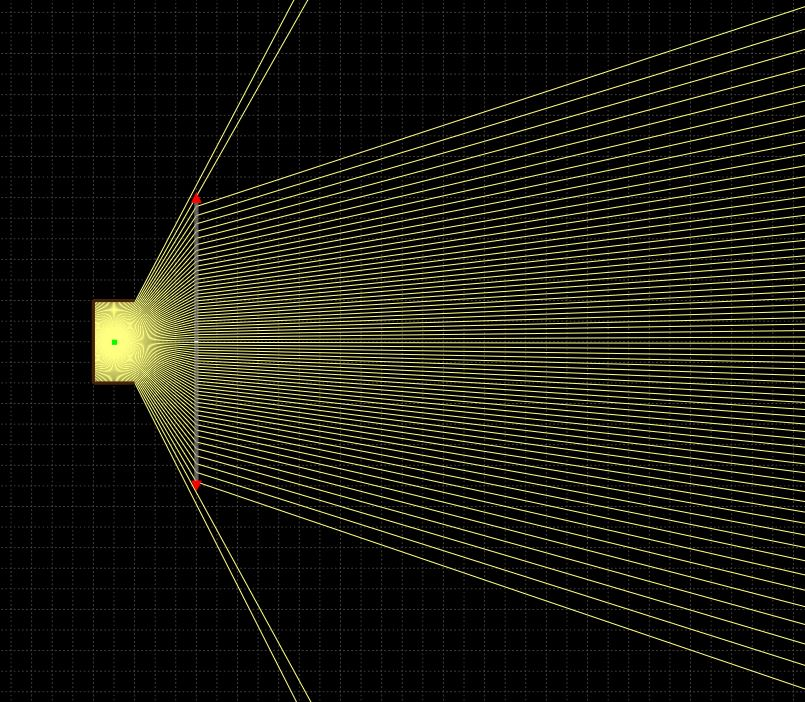
\includegraphics[width=.9\linewidth]{figures/litreview/lens_divergent_beam.JPG}
		\captionof{figure}{Divergent}
		\label{fig:lens_divergent}
	\end{minipage}%
	\begin{minipage}{.3\textwidth}
		\centering
		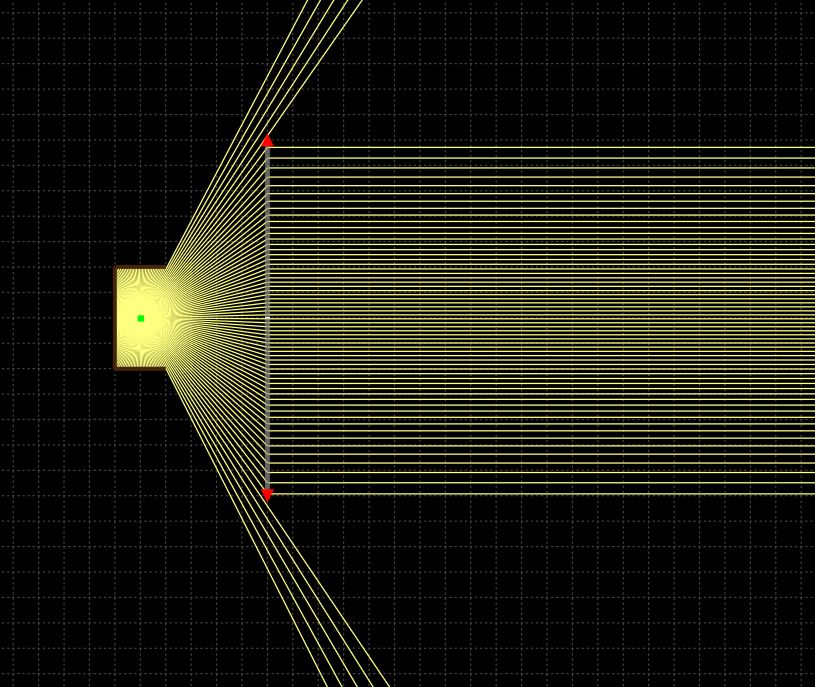
\includegraphics[width=.9\linewidth]{figures/litreview/lens_parallel_beam.JPG}
		\captionof{figure}{Parallel}
		\label{fig:lens_parallel}
	\end{minipage}
	\begin{minipage}{.3\textwidth}
		\centering
		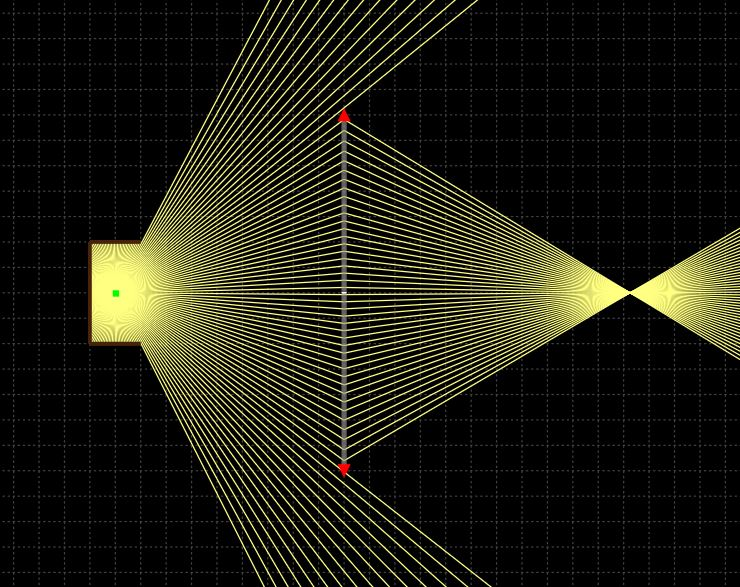
\includegraphics[width=.9\linewidth]{figures/litreview/lens_focus_beam.JPG}
		\captionof{figure}{Convergent}
		\label{fig:lens_convergent}
	\end{minipage}
	\caption*{Images showing the different behaviours of light interacting with a lens}
\end{figure}

Figures \ref{fig:lens_divergent} to \ref{fig:lens_convergent} illustrate\footnotemark the three behaviours that may be achieved using a single point source of light and an ideal lens. Behavious in figure \ref{fig:lens_divergent} occurs when a point light source exists between the near focal point and the lens, the resulting beam of light diverges after passing through the lens. Figure \ref{fig:lens_parallel} shows that for a light source placed at the focal point, the rays of light will emerge from the lens parallel. Finally \ref{fig:lens_convergent} illustrates that for a point source of light placed further beyond the near focal point (on the opposite side to the lens) results in a beam that initially converges, focusing to some point and then diverges.
\footnotetext{Created using \href{https://ricktu288.github.io/ray-optics/simulator/}{Ray-Optics Simulator}}

In may cases including this investigation, the light coming from an LED may be approximated as a point source and the lens approximated as ideal.


\subsection{IR Communication}
%This is where I talk about different IR protocols

IR has is used in many applications, this is because it is cheap, efficient and simple to use. A basic implementation can be done using an IR LED, IR receiver IC and a pair of microcontrollers.

There are several IR communication protocols in existence. Of the extensive list of available protocols the following are quite popular

\begin{itemize}
	\item RC-5
	\item RC-6
	\item NEC
	\item SIRC
\end{itemize}

Practically all the IR protocols for remote control applications follow the exact same principles for encoding and transmitting information through IR radiation. To transmit information, an IR LED is modulated at a particular carrier frequency (usually around 36kHz). Modulation is necessary because there are many sources of IR radiation and it would be otherwise impossible to distinguish the user generated IR signal from surrounding noise sources. Each protocol defines specific timing conditions for how long the IR radiation should be modulated to portray a specific symbol. This is where the various protocol differ.

Some protocols use a technique known as pulse width encoding. This technique involves modulating the IR LED for a different period of time depending on whether a 1 or 0 is to be transmitted, while maintaining a constant period of time between transmissions. This is the technique is incorporated into Sony's SIRC protocol.

Other protocols use pulse distance encoding, such as the NEC protocol by Renesas. This protocol involves modulating the IR LED for a fixed period of time and the time period between each modulation is used to indicate either a 1 or 0.

Finally, some of the IR protocols use Manchester Encoding to embed information, such as in the case of the very popular RC-5 protocol and its successor the RC-6 protocol. Due to its wide adoption and popularity, as well as incorporation of the elegant Manchester Encoding technique, it was decided to use an adaption of the RC-5 protocol in this project. A review of Manchester Encoding is detailed in section \ref{sec:manchester_encoding} below.

\subsubsection{RC-5 Protocol}
This project uses a slightly modified version of the RC-5 transmission protocol. The the original RC-5 protocol is illustrated in figure \ref{fig:rc_5_protocol}. The bits are encoded using the IEEE 802.3 convention for Manchester Encoding. The modulation frequency of the carrier is 36kHz and the length of one bit period is 64 cycles or 1.778mS.

\begin{figure}[H]
	\centering
	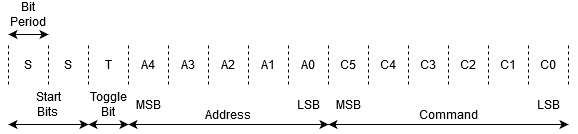
\includegraphics[width=0.8\linewidth]{figures/litreview/rc5_protocol.png}
	\caption{RC-5 IR Protocol}
	\label{fig:rc_5_protocol}
\end{figure}

Every transmission begins with two start bits, these bits always have a value of 1. Following the start bits is a 'toggle' bit. In remote control applications it is sometimes important to distinguish between a button remaining depressed and a button being repeatedly pressed.

This is achieved through the toggle bit, which remains constant

When a button is depressed, the message is transmitted repeatedly with a 114ms gap between transmissions.


\subsection{Materials Interaction}
This is where I talk about materials that block visible light but let IR through

%%%%%%%%%%%%%%%%%%

\section{Reliable Communication}

\subsection{Noise in Air}
Talk about interference and noise due to ambient light

\subsection{Modulation}
Talk about modulation to allow for easy detection

\subsection{Manchester Encoding}
\label{sec:manchester_encoding}
Manchester Code is a type of phase encoding. It is classified as a line code and is produced by generating patterns through some measurable phenomena. The commonly used mediums to represent a Manchester encoded signal would be voltage, current and light (electromagnetic radiation).

Manchester coding, as its name suggests, was developed at the University of Manchester and it was first published in 1949 \cite{Jameel2019}. Manchester encoding is a protocol for integrating the clock and data into a single sequence consisting of only two symbols. It does not require clock synchronization, only that a predefined bit-width is known by both the receiver and transmitter. 

The principle behind Manchester code is to encode the information into transitions between two symbols. This technique makes the encoding scheme particularly useful in communication by means of inductive coupling such as in RFID. Due to its self-clocking property and simplicity it is the standard means of encoding for many IR applications. Perhaps the most common application is in the remote controls we use for various appliances.

Manchester code is a special form of binary phase shift keying (BPSK). A square wave of a particular frequency is chosen as the carrier and binary information is encoding by adjusting the setting a phase off set to either 0\degree or 180\degree s. In figure \ref{fig:manchesterencoding} the process of encoding 10 bits is illustrated. Two conventions exist, their difference lies solely in the definition of which logic values are represented by each of the two transitions. The convention used throughout this investigation is in accordance to the IEEE 802.3 standard which defines a logical 1 as the transition from 0 to 1 and a zero as 1 to 0. The other convention used by inventor G.E. Thomas is the inverse of this and is also widely used.\\

\begin{figure}[H]
	\centering
	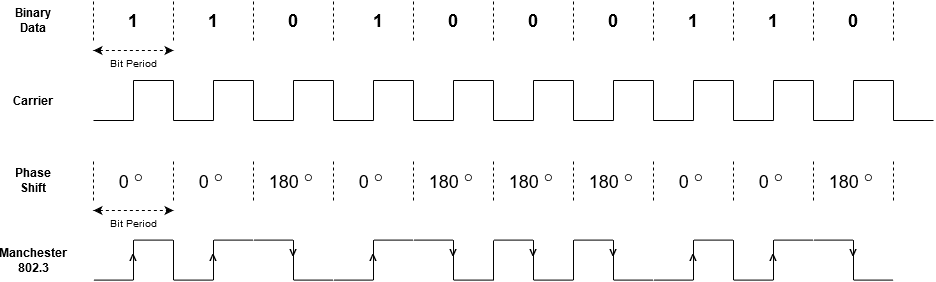
\includegraphics[width=0.7\linewidth]{figures/litreview/manchester_encoding}
	\caption{Manchester code example using 10 bits}
	\label{fig:manchesterencoding}
\end{figure}

\subsubsection{Encoding Algorithm}


\subsubsection{Decoding Algorithm}
Different techniques have been developed to decode Manchester encoded sequences. In his paper on methods for decoding Manchester code, R. A. Dobre discusses an elegant and widely used finite state machine approach which has been illustrated in figure \ref{fig:manchesterdecodingfsm} below. \cite{Dobre2014}

\begin{figure}[H]
	\centering
	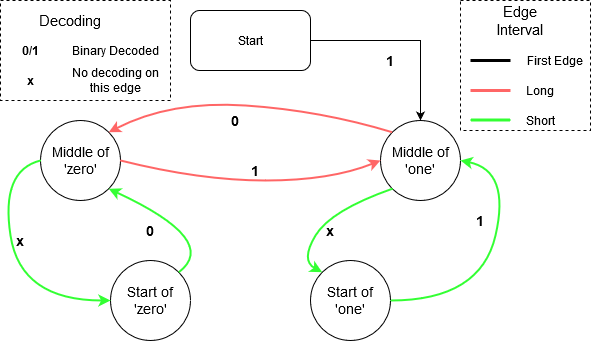
\includegraphics[width=0.7\linewidth]{figures/litreview/manchester_decoding_fsm.png}
	\caption{FSM Algorithm for Decoding Manchester Sequences}
	\label{fig:manchesterdecodingfsm}
\end{figure}

The state machine approach is particularly useful because it only considers the time period between the current detected edge and the previous edge. It removes the need to track samples saving on memory and reducing processing power requirements, all without introducing additional complexity.

It should be noted that this FSM assumes the first bit transmitted is always a logical 1. In addition does not detect the end of a sequence, so additional logic is required such as a counter to detect when a certain number of bits have been received or by means of implementing timeout detection.

%\iffalse
\subsection{Error Control}

In information theory, error control is the field of study that concerns issues of detecting errors in digital communications and in certain instances provides the means to corrected these errors. Whenever data is transmitted over some kind of network, there is the possibility that interference can cause a bit to flip resulting in an error. Richard Hamming pioneered in the development of digital error control and is known for (amongst other things) the Hamming code.

Various ways to detect and potentially correct the presence of an error. The most trivial technique known as a 'repetition code' simply involves sending the information three times, making it possible to detect if one of the three data-streams doesn't match the others. Although repetition codes allows for both error detection and correction, it is horribly inefficient. Various techniques have been developed and each technique balances complexity and efficiency.

\subsubsection{Parity}
Using a parity bit is the most simple means to detect an error in a bit sequence. The parity of a sequence may be defined as the result of a bit wise exclusive or (XOR) operation, this is known as 'even parity' because the parity bit value is chosen such that upon appending it to the bit-sequence there would be an even number of 1s. Conversely 'odd parity' calculates the parity bit such the number of 1s in the generated sequence is odd. Table \ref{tbl:party_examples} below provides example bit sequences and the respective even (given by the XOR operation) and odd parity values.

\begin{table}[H]
	\centering
	\begin{tabular}{ccc}
		\hline
		\multicolumn{1}{l}{\textbf{Bit Sequence}} & \textbf{XOR of Bits} & \multicolumn{1}{l}{\textbf{Odd Parity Bit}} \\ \hline
		0000000 & 0 & 1 \\ \hline
		1111111 & 1 & 0 \\ \hline
		1010101 & 0 & 1 \\ \hline
		1001100 & 1 & 0 \\ \hline
	\end{tabular}
	\caption{Even and odd parity for example bit sequences}
	\label{tbl:party_examples}
\end{table}

 To use parity as a method to detect errors, the sender and receiver choose to use either even or odd parity. Before transmission, the sender calculates the parity bit for the sequence to be sent, this bit is then appended to the bit-stream. Upon receiving the bit-stream, the same parity calculation is done on the sequence. If the result of this calculation is a 1 it can be said for certain that an error occurred, if the result is zero it can be said that no error occurred or an even number of errors occurred.

%\subsubsection{Hamming Code}

%\fi


\subsection{Demodulation}
Need to talk about demodulating, Goertzel, DSP, tone-detectors


%%%%%%%%%%%%%%%%%%
\section{Digital Signal Processing}
In the age of micro-controllers and micro-processors, in many situations it has become far more effective to use digital signal processing to manipulate and processes signals.

Part of the IR decoding process requires detecting the presence of a particular frequency (commonly referred to as a tone). The natural tool to turn to when examining the frequency content of a signal is the discrete Fourier transform (DFT). The DFT is well established and there exist a variety of algorithms which compute its values, perhaps the most well known being the FFT. However, for the purposes of detecting a single tone of a predetermined frequency, the DFT is not the most efficient method, even when optimized algorithms such as the FFT are implemented.

The FFT provides a very efficient means for determining all the DFT coefficients, but in a use case only a few of the coefficients are used and the rest discarded it is not the most efficient technique. By using a less efficient process for calculating individual coefficients of the DFT it is possible to greatly reduce program complexity and processing time relative to an implementation that uses the FFT.

\subsection{Goertzel Algorithm}

The algorithm which computes individual DFT coefficients is known as the Goertzel algorithm (or Goertzel Filter) and was developed by G. Goertzel in 1958. \cite{Goertzel1958} A common application of the Goertzel algorithm is in the decoding of DTMF\footnotemark{} signals.
\footnotetext{Duel Tone Multiple Frequency}

\subsubsection{Derivation}
The goertzel algorithm may be derived from the formula for the DFT. In the derivation \(W_N = e^{-j\frac{2\pi}{N}}\).

\begin{equation}
	\label{eqn:dft_defn}
	X[k] = \sum_{n=0}^{N-1}x[n]W_{N}^{nk}
\end{equation}

Multipling the right side of equation \ref{eqn:dft_defn} by \(W_{N}^{-Nk} = e^{j\frac{2\pi N k}{N}} = 1\) we get

\begin{equation}
X[k] = W_{N}^{-Nk}\sum_{n=0}^{N-1}x[n]W_{N}^{nk}
\end{equation}

Rearranging we get

\begin{equation}
\label{eqn:dft_conv}
X[k] = \sum_{n=0}^{N-1}x[n]W_{N}^{k(n-N)}
\end{equation}

Notice that if we consider the signal \(h_k[l] = W_N^{-kl}u[l]\), then equation \ref{eqn:dft_conv} is the convolution of $h_k[l]$ with $x[l]$. Substituting these signals into equation \ref{eqn:dconv} (formula for discrete convolution) below, we can rearrange the result to arrive at equation \ref{eqn:dconv_sub}.

\begin{equation}
	\label{eqn:dconv}
	y_k[l] = \sum_{m=0}^{N-1}x[m]h_k[l - m]
\end{equation}

\begin{equation}
	\label{eqn:dconv_sub}
y_k[l] = \sum_{m=0}^{N-1}x[m]W_N^{k(m-l)}
\end{equation}

Comparing equation \ref{eqn:dft_conv} with equation \ref{eqn:dconv_sub}, it becomes clear that from the convolution $y_k[n] = x[n] * h_k[n]$ we can find the value of $X[k]$ by substituding N into $y_k[n]$. Thus the following relationship exists

\begin{equation}
\label{eqn:goertzel_relationship}
X[k] = y_k[N]
\end{equation}

%%%%
%Now deriving the filter
%%%%

In their paper on generalizing the Goertzel algorithm for non-integer multiples of the the fundamental frequency, P. Sysel and P. Rajmic show how the function $h_k[n]$ may be transformed to the Z-domain and optimized to reduce the amount of computational power required to compute the DFT coefficient \cite{Sysel2012}. The results are given by the following equations.

%The following equations are taken from the paper - check if thats okay with Simon...
\[h_k[n] \xRightarrow{\text{Z}} H_k(z)\]

\begin{equation}
W_N^{-kl}u[n] \xRightarrow{\text{Z}} \frac{1}{1 - W_N^{-k}z^{-1}} = \frac{1}{1 - e^{j\frac{2\pi k}{N}}z^{-1}}
\end{equation}

$H_k(z)$ can then be manipulated to give

\begin{equation}
\label{eqn:g_optimized_ir}
H_k(z) = \frac{1 - e^{-j\frac{2\pi k}{N}}z^{-1}}{1 - 2cos(\frac{2\pi k}{N})z^{-1} + z^{-2}}
\end{equation}

Finally, equation \ref{eqn:g_optimized_ir} can be converted to state variable form to yeild the following


\begin{equation}
	\label{eqn:g_ss}
	s[n] = x[n]+2cos(\frac{2\pi k}{N})s[n-1]-s[n-2]
\end{equation}


\begin{equation}
	\label{eqn:g_ssoutput}
	y_k[n] = s[n]-e^{-j\frac{2\pi k}{N}}s[n-1]
\end{equation}



\subsubsection{Implementation}
\label{sec:goertzel_implementation}
Using the state variable equations \ref{eqn:g_ss} and \ref{eqn:g_ssoutput} we can implement the goertzel filter digitally. The following code in listing \ref{lst:goertzel_algorithm} shows a Goertzel filter implemented in the Octave environment.

\begin{lstlisting}[caption={Goertzel Algorithm - Octave Implementation\label{lst:goertzel_algorithm}}]
function magnitudesqd = calculate_goertzel (N, bin_frequency, sampling_frequency, samples)

	k = round(N*bin_frequency/sampling_frequency);
	omega = (2*pi*k)/N;
	cosval = cos(omega);
	sinval = sin(omega);
	coeff = 2*cosval;
	
	s1 = 0;
	s2 = 0;
	
	for i = 1:N
	s0 = (samples(i) + (coeff*s1) - s2);
	s2 = s1;
	s1 = s0;    
	end
	
	realv = (s1 - (s2 * cosval));
	imgv = (s2 * sinval);  
	
	magnitudesqd = realv*realv + imgv*imgv;

endfunction
\end{lstlisting}

\subsubsection{Nyquist-Shannon}

\[f_{Nyquist} = \frac{f_{sampling}}{2}\]

\begin{equation}
\label{eqn:sampling_frequency}
BW < f_{Nyquist}
\end{equation}




%%%%%%%%%%%%%%%%%%

\section{IR Radiation}
This is where I talk about the section of the EM spectrum that is IR


\subsection{IR Radiation Detection}

Photodiodes and transistors




%%%%%%%%%%%%%%%%%%

\section{Recreational Electronics}


\subsection{Recreational Laser Use}

\section{Microcontrollers}
Histroy of how uc have come down in price making them a viable component in hobby electronics.

\subsection{ADC}

\subsection{Timers}
PWM

\subsection{Libraries - The HAL Library}


%%%%%%%%%%%%%%%%%%

\section{Pulse Width Modulation}







